\documentclass[11pt,a4paper]{article}
\usepackage[margin=2.35cm]{geometry}
\usepackage{setspace}
\setstretch{1.22}
\usepackage{amsmath,amssymb}
\usepackage{booktabs}
\usepackage{pgfplots}
\pgfplotsset{compat=1.18}
\usepackage[hidelinks]{hyperref}
\setlength{\parskip}{0.32em}
\setlength{\parindent}{1.05em}
\pgfplotsset{every axis/.append style={tick label style={font=\small},label style={font=\small}}}

\title{A Deep Network for Threshing Efficiency\\and Mechanical Stability}
\author{A short computer-science paper on the command model\\of a thesis on thresher efficiency}
\date{}

\begin{document}
\maketitle
\thispagestyle{empty}

\begin{abstract}
\noindent
A numerical optimizer can raise grain recovery on a thresher if it is given the true feed, the true moisture, and a free solve. An onboard program gets a noisy sensor window and a deadline. This paper trains a feedforward network to imitate that optimizer. The inputs are the window features of a four-station placement. The outputs are four normalized setpoints: intensity, residence, cleaning, and feed admission. The teacher maximizes recovery with explicit prices on energy, impurity, breakage, and a stability floor at \(0.70\). On a weighted seasonal mix the network lowers grain loss from \(2.85\%\) at a fixed setting and \(2.50\%\) on a moisture card to \(1.80\%\), against \(1.78\%\) for the teacher. Specific energy rises from \(1.41\) to \(1.63\,\mathrm{kWh\,t^{-1}}\). A linear imitator on the same features reaches \(1.88\%\). Depth is a small gain on the command and a large gain on the companion status task. A rate-limited transient holds the stability floor while the feed crests. The study is a numerical experiment, not a field trial.
\end{abstract}

\section{Introduction}

Published combine controllers move one or two actuators from a moisture signal, a loss sensor, or a short predictive model \cite{craessaerts2010,coen2008,chen2025}. A moisture card is the simplest of these policies, and it is not foolish: wetter grain is given a harder and a longer pass. It cannot see a product of feed and moisture, and it cannot see an axial load that is heavy only at the inlet. An optimizer that sees both will spend residence on a wet, heavy crop and will refuse that spend on a light crop, because breakage and energy are in the cost. The optimizer is too slow, and too dependent on the true disturbance, to be the program that runs every control step \cite{nocedal2006,rawlings2017}.

This paper is the command half of a computer-science thesis. A companion paper places the sensors and identifies a discrete operating status. The command network does not read that label. It reads the same features and emits a command. Imitation is used because a teacher is available from the simulator. A policy search without a teacher would be a different algorithm.

\section{Teacher and network}

The plant is static and reduced-order. Admitted feed is \(q_e=q(0.82+0.18\,u_F)\), so the feed command is a trim. Recovery is
\begin{equation}
\eta=(q_e/q)\,(1-L),
\label{eq:eta}
\end{equation}
with \(L\) the sum of unthreshed, free-grain, and sieve losses. Cutting the trim lowers \(\eta\). A policy cannot look efficient by refusing crop. Packing,
\begin{equation}
\pi \propto \max(q_e/6-0.75,\ 0)\,\max(m-0.16,\ 0),
\label{eq:pack}
\end{equation}
is zero unless the feed is heavy and the crop is wet, and it multiplies unthreshed loss until residence rises. A card that is linear in moisture does not contain \(\pi\).

The teacher maximizes
\begin{equation}
\begin{aligned}
J=\eta&-0.012\,e-0.48\,\iota-1.15\,b-0.025\,\mathrm{CV}\\
&-0.26\max(0,\ 0.70-S)
-0.40\max(0,\ F_{\max}/1680-0.82)^2
\end{aligned}
\label{eq:J}
\end{equation}
over the unit box, from a four-level grid and a bound-constrained polish \cite{nocedal2006}. Here \(e\) is specific shaft energy, \(\iota\) impurity, \(b\) a breakage index that grows with residence and intensity, \(\mathrm{CV}\) the coefficient of variation of eight station loads, and \(S\in[0,1]\) a stability index. The stability term is a hinge. Above \(0.70\) the teacher may spend calmness it does not need. The fixed baseline is \((u_I,u_R,u_C,u_F)=(0.50,0.44,0.46,1)\). The card raises the first three components with moisture and leaves the trim open. It does not read \(q\).

Features are the \(23\)-dimensional window statistics of stations \(1,4,5,8\) plus torque, vibration, a loss proxy, return flow, power, moisture, and feed. The network is \(23\)--\(64\)--\(64\)--\(32\)--\(4\), ReLU hidden units, linear output clipped to \([0,1]\), \(7908\) parameters, \(7744\) multiply-adds \cite{goodfellow2016,he2015}. Training is squared error against the teacher's command, Adam at learning rate \(10^{-3}\), \(140\) epochs, best validation epoch \(122\) \cite{kingma2015}. Each disturbance contributes three windows, drawn under the card, under a random command, and under the fixed setting, all labeled with the same teacher command. One mixture is the whole adaptation to the deployment distribution \cite{ross2011}. The linear ablation is least squares on the same standardized features.

The onboard step standardizes the window, evaluates the net, and limits each component's change to \(0.08\) per \(0.2\,\mathrm{s}\). If the companion status net is below confidence \(0.55\), the step writes the card instead. The seasonal table does not use that gate. It is the network with a full window.

\section{Seasonal evaluation}

Eight steady points, wheat-heavy and with rice and soybean included, are weighted to one. Table~\ref{tab:season} is the mean. The network is within \(0.03\) points of the teacher's loss and within a few hundredths of the teacher's energy, impurity, and breakage. The linear imitator recovers most of the gain and leaves \(0.08\) points more loss. The card beats the fixed setting by \(0.35\) points and is not a dummy baseline.

\begin{table}[ht]
\centering
\caption{Weighted seasonal means. Loss, impurity, and breakage are percent. Energy is \(\mathrm{kWh\,t^{-1}}\).}
\label{tab:season}
\begin{tabular}{@{}lrrrrr@{}}
\toprule
Quantity & Fixed & Card & Linear & Network & Teacher \\
\midrule
Grain loss & 2.85 & 2.50 & 1.88 & 1.80 & 1.78 \\
Recovery & 97.15 & 97.50 & 98.07 & 98.13 & 98.22 \\
Impurity & 1.17 & 1.20 & 1.50 & 1.50 & 1.50 \\
Breakage & 1.04 & 1.17 & 1.43 & 1.49 & 1.51 \\
Specific energy & 1.41 & 1.47 & 1.60 & 1.63 & 1.64 \\
Stability \(S\) & 0.686 & 0.696 & 0.702 & 0.701 & 0.700 \\
\bottomrule
\end{tabular}
\end{table}

The mean hides two rows that decide whether the imitator understood \(J\). On dry, heavy wheat the card is worse than the fixed setting, because low moisture eases the card while the feed stays heavy: loss \(2.85\%\) against \(2.65\%\). The teacher moves residence up to \(0.59\) and holds intensity at \(0.50\), with loss \(1.96\%\) and breakage \(1.27\%\). The network overshoots, writes residence \(0.71\) and intensity \(0.59\), and records loss \(1.57\%\) with breakage \(1.63\%\). A loss-only ranking would put the network ahead of the teacher. The objective does not. On wet rice the fixed loss is \(4.99\%\) at stability \(0.54\) and a peak load of \(1441\,\mathrm{N}\). The network reaches stability \(0.70\), peak \(1182\,\mathrm{N}\), and loss \(2.65\%\), short of the teacher's \(2.27\%\). Residence is \(0.80\) against the teacher's \(0.85\). The load coefficient of variation falls from \(0.157\) to \(0.047\). On light wheat both the teacher and the network lower residence, to about \(0.38\), and spend stability from \(0.76\) down to the floor. Holding every crop longer is not the policy.

Feed admission stays at one on every weighted point. The trim is available. The teacher meets the blockage hinge with residence and intensity, and the network copies that choice. Recovery and the complement of loss therefore move together.

On an i.i.d.\ test mixture, wider than the season, network and linear loss both sit at \(1.95\%\), with the teacher at \(1.98\%\) because \(J\) is not pure loss. Command mean absolute error is \(0.022\) for the network and \(0.023\) for the linear map. The tenth percentile of stability rises from \(0.51\) at the fixed setting to \(0.69\) for the network, against \(0.70\) for the teacher. Thirty percent of network test windows still fall just under the floor. The executive does not project the command back onto the hinge. That projection would be the teacher, called at runtime.

\section{A feed transient}

Wheat at moisture \(0.17\) is held at \(5\,\mathrm{kg\,s^{-1}}\) except for a crest of about \(8.2\,\mathrm{kg\,s^{-1}}\) at \(t=12\,\mathrm{s}\). The network starts on the card and is rate-limited. Figure~\ref{fig:slug} is the peak load. At the crest the fixed command reaches \(1367\,\mathrm{N}\) and \(3.19\%\) loss. The network reaches \(1118\,\mathrm{N}\) and \(1.81\%\) loss, with residence \(0.84\) and stability still at \(0.70\). Mean loss over \(26\,\mathrm{s}\) is \(2.59\%\), \(2.38\%\), and \(1.48\%\) for the fixed command, the card, and the network. At \(t=0\) the network has not moved, which is the check that the crest result is not a warm start from the teacher.

\begin{figure}[ht]
\centering
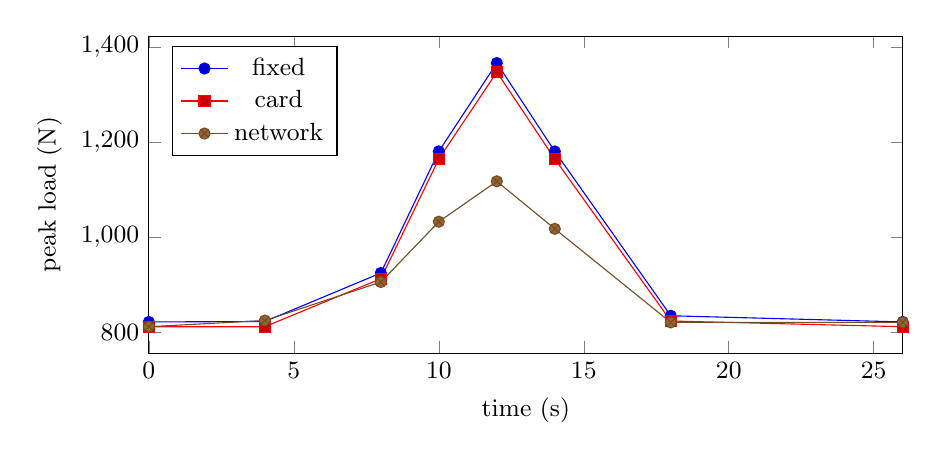
\begin{tikzpicture}
\begin{axis}[
  width=0.92\textwidth, height=5.6cm,
  xlabel={time (s)}, ylabel={peak load (N)},
  xmin=0, xmax=26,
  legend style={font=\small,at={(0.03,0.97)},anchor=north west},
]
\addplot coordinates {(0,822) (4,823) (8,925) (10,1181) (12,1367) (14,1181) (18,835) (26,822)};
\addplot coordinates {(0,812) (4,812) (8,913) (10,1165) (12,1348) (14,1165) (18,824) (26,812)};
\addplot coordinates {(0,812) (4,825) (8,906) (10,1033) (12,1118) (14,1018) (18,821) (26,821)};
\legend{fixed,card,network}
\end{axis}
\end{tikzpicture}
\caption{Peak station load on the wheat transient. The network is rate-limited and starts equal to the card.}
\label{fig:slug}
\end{figure}

\section{Conclusion}

The command this plant requires is an imitation of a priced optimizer, not a second moisture card. A network of a few thousand parameters matches the teacher's seasonal loss and copies the teacher's prices, including the prices that make a low-loss overshoot on dry, heavy wheat a worse command. A linear map on the same features is close. The depth that clearly changes a score in the parent thesis is the status classifier, not this command head. The transient shows that a rate limit of the size an actuator can follow is enough for a crest a few seconds wide. Nothing in the tables is a measured field loss. The tables say what this cost, this teacher, and this imitator do on the simulator that defines them.

\begin{thebibliography}{9}
\bibitem{craessaerts2010}
G.~Craessaerts, J.~De~Baerdemaeker, B.~Missotten, and W.~Saeys,
``Fuzzy control of the cleaning process on a combine harvester,''
\emph{Biosystems Engineering}, vol.~106, no.~2, pp.~103--111, 2010.
\bibitem{coen2008}
T.~Coen, W.~Saeys, B.~Missotten, and J.~De~Baerdemaeker,
``Cruise control on a combine harvester using model-based predictive control,''
\emph{Biosystems Engineering}, vol.~99, no.~1, pp.~47--55, 2008.
\bibitem{chen2025}
Z.~Chen, Z.~Qian, C.~Jin, and T.~Yang,
``Research progress on control algorithms for grain combine harvesters,''
\emph{Applied Sciences}, vol.~15, no.~16, art.~9176, 2025.
\bibitem{nocedal2006}
J.~Nocedal and S.~J. Wright, \emph{Numerical Optimization}, 2nd~ed. Springer, 2006.
\bibitem{rawlings2017}
J.~B. Rawlings, D.~Q. Mayne, and M.~M. Diehl,
\emph{Model Predictive Control}, 2nd~ed. Nob Hill, 2017.
\bibitem{ross2011}
S.~Ross, G.~J. Gordon, and J.~A. Bagnell,
``A reduction of imitation learning and structured prediction to no-regret online learning,''
in \emph{Proc. AISTATS}, 2011, pp.~627--635.
\bibitem{goodfellow2016}
I.~Goodfellow, Y.~Bengio, and A.~Courville, \emph{Deep Learning}. MIT Press, 2016.
\bibitem{he2015}
K.~He, X.~Zhang, S.~Ren, and J.~Sun,
``Delving deep into rectifiers,''
in \emph{Proc. ICCV}, 2015, pp.~1026--1034.
\bibitem{kingma2015}
D.~P. Kingma and J.~Ba,
``Adam: A method for stochastic optimization,''
in \emph{Proc. ICLR}, 2015.
\end{thebibliography}

\end{document}
